%2.3- The paper should also discuss subsequent adjustments to the policy in 2007, and the potential disruption created by the 2010 earthquake. Both could have affected treatment quality/intensity (or even the different components?) as well as local perceptions, and it is important to explain how these events are handled in the empirical section. For example, is it possible to exclude the affected areas, or to test whether the earthquake generated changes in perceptions that confound the results? At the same time, could the 2007 adjustment and 2010 earthquake be exploited as sources of heterogeneity to shed light on mechanisms if they were different in nature?

In 2007, an evaluation conducted by DIPRES (Chile's Directorate of Budget, an independent government body) recommended the formalization of new specialized roles within each police station, including a Head of Operations Office, a Community Affairs Officer, and officers responsible for drug prevention, domestic violence, and judicial orders \citep{DIPRES2007_largo}. However, these changes were more formal than operational, and were not effectively implemented at scale until the introduction of \emph{Plan Cuadrante 2.0}, outside our study period. The 2014 DIPRES evaluation documents, for example, that while the Community Affairs Officer role was formally created in some municipalities, dedicated personnel and budget were not assigned, and the community integration model (MICC) was only piloted in 4 to 6 police stations in 2012--2013 (none of these stations were in municipalities in our analytical sample) before its financing agreement was discontinued in early 2014 \citep{DIPRES2014,Manual_Carabineros2018}. Similarly, the Operations Office lacked the digitalization, personel, and dedicated resources needed to fulfill its analytical functions until the launch of \emph{Plan Cuadrante 2.0} \citep{DIPRES2014, Manual_Carabineros2018}. Our results therefore capture the effects of the original \emph{Plan Cuadrante}, characterized primarily by the reduction of police catchment areas and the permanent territorial assignment of officers, without contamination from the more substantive operational reforms introduced later.

Regarding the disruption that the 2010 earthquake in Concepcion could have on the implementation of \emph{Plan Cuadrante}: The 2010 earthquake halted the expansion of the program. No new municipalities joined the program in 2010. Moreover, it could potentially confound our estimates on outcomes if it differentially affected treated and control municipalities, either by disrupting police operations and thus reducing treatment intensity, or by independently affecting crime perceptions and security outcomes in ways unrelated to \emph{Plan Cuadrante}. To address this concern, in the revised manuscript we re-estimate our main results excluding municipalities more exposed to the earthquake, defined as those experiencing a Modified Mercalli Intensity greater than 7. This corresponds to 21 municipalities in the ENUSC sample and 158 municipalities in the administrative data sample. The results, reported in Figure \ref{fig:figure02_noEQ}, are nearly identical to the main estimates, suggesting that the 2010 earthquake does not confound our estimates.

We have added the following footnote in Section 4.1 of the updated manuscript:

\begin{adjustwidth}{2em}{0em}
These results are robust to excluding municipalities most affected by the 2010 Maule earthquake, defined as those with a Modified Mercalli Intensity greater than 7; see Figure \ref{fig:figure02_noEQ} in Online Appendix \ref{sec:appendixC} for details.
\end{adjustwidth}

We also add the following subsection, ``Robustness to the 2010 Earthquake,'' to Online Appendix C reporting this exercise in detail:

\begin{adjustwidth}{2em}{0em}
The 2010 Maule earthquake could confound our estimates if it differentially affected treated and control municipalities, either by disrupting police operations and thus reducing treatment intensity, or by independently affecting crime perceptions and security outcomes in ways unrelated to \emph{Plan Cuadrante}. To address this concern, we re-estimate our main results excluding municipalities more exposed to the earthquake, defined as those experiencing a Modified Mercalli Intensity greater than 7. This corresponds to 21 municipalities in the ENUSC sample and 158 municipalities in the administrative data sample. The results, reported in Figure \ref{fig:figure02_noEQ}, are nearly identical to the main estimates, confirming that the 2010 earthquake does not drive our findings.
\end{adjustwidth}

Regarding the suggestion to exploit the earthquake as a source of heterogeneity, we agree this is an interesting analysis that might help shed light on the mechanisms. To assess the heterogeneous effects of \emph{Plan Cuadrante} by exposure to the earthquake, we estimate the effects of the program separately for municipalities more exposed to the earthquake (Modified Mercalli Intensity greater than 7) and municipalities with a Modified Mercalli Intensity of 7 or lower. The results are reported in Figure \ref{fig:heterogeneity_earthquake_mmi}. They show relatively similar effects across the two groups for both victimization and crime perception. The effects on investment in security measures and reported crime appear somehow larger for municipalities less exposed to the earthquake, although they remain statistically significant for the more affected municipalities as well.



\clearpage
\noindent\textbf{Other figure referenced above:}
\vspace{0.5em}

{\renewcommand{\thefigure}{C.11}
%--- Robustness check: 2010 Maule earthquake (Mercalli > 7 excluded)
\begin{figure}[h!]
    \centering
    \caption{Effects of \emph{Plan Cuadrante} excluding Municipalities Affected by the 2010 Earthquake}
    \label{fig:figure02_noEQ}
    \begin{subfigure}{0.495\textwidth}
        \centering
        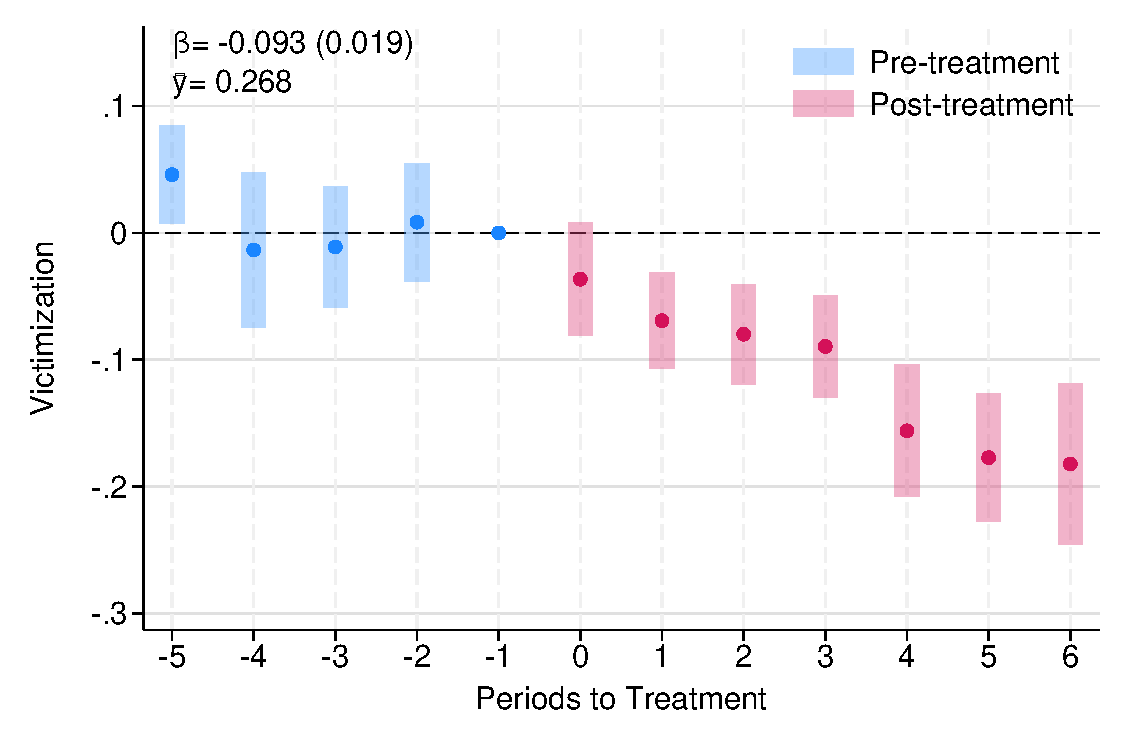
\includegraphics[width=\textwidth]{../manuscript/Graphs/results_victimization_noEQ.pdf}
        \caption{Victimization in last 12 months}
    \end{subfigure}%
    ~
    \begin{subfigure}{0.495\textwidth}
        \centering
        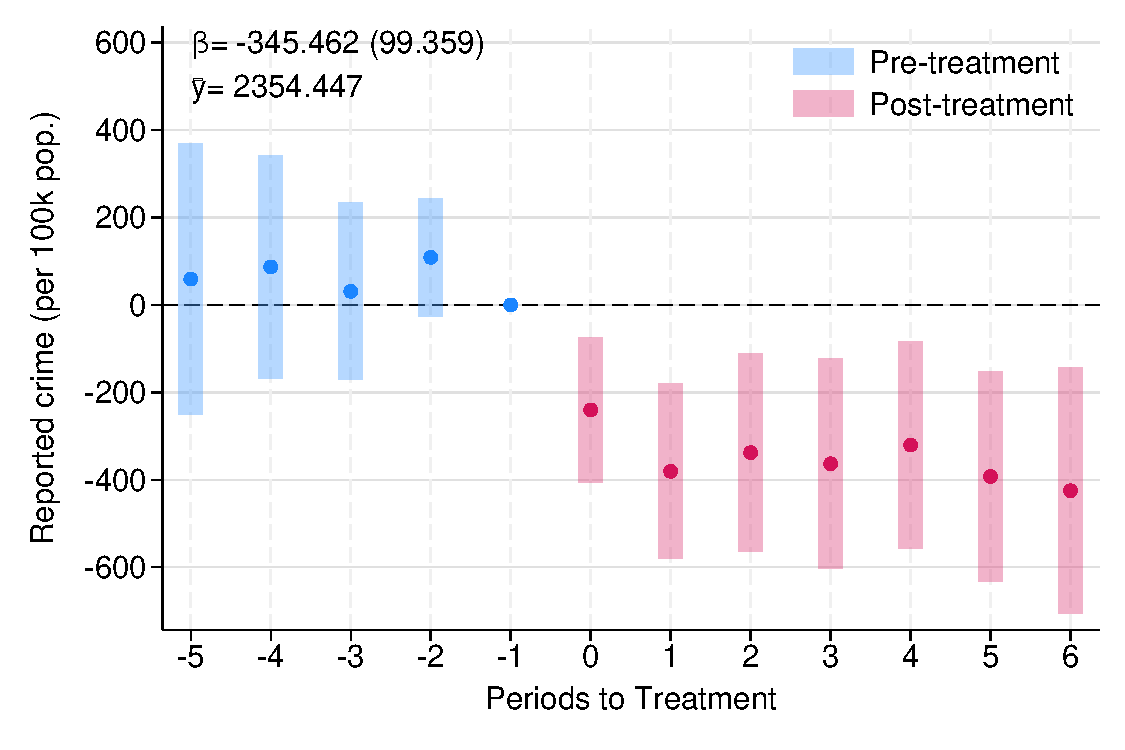
\includegraphics[width=\textwidth]{../manuscript/Graphs/totalreportedcrime_allcomunas_noEQ.pdf}
        \caption{Reported crime per 100k inhabitants}
    \end{subfigure}
    \begin{subfigure}{0.495\textwidth}
        \centering
        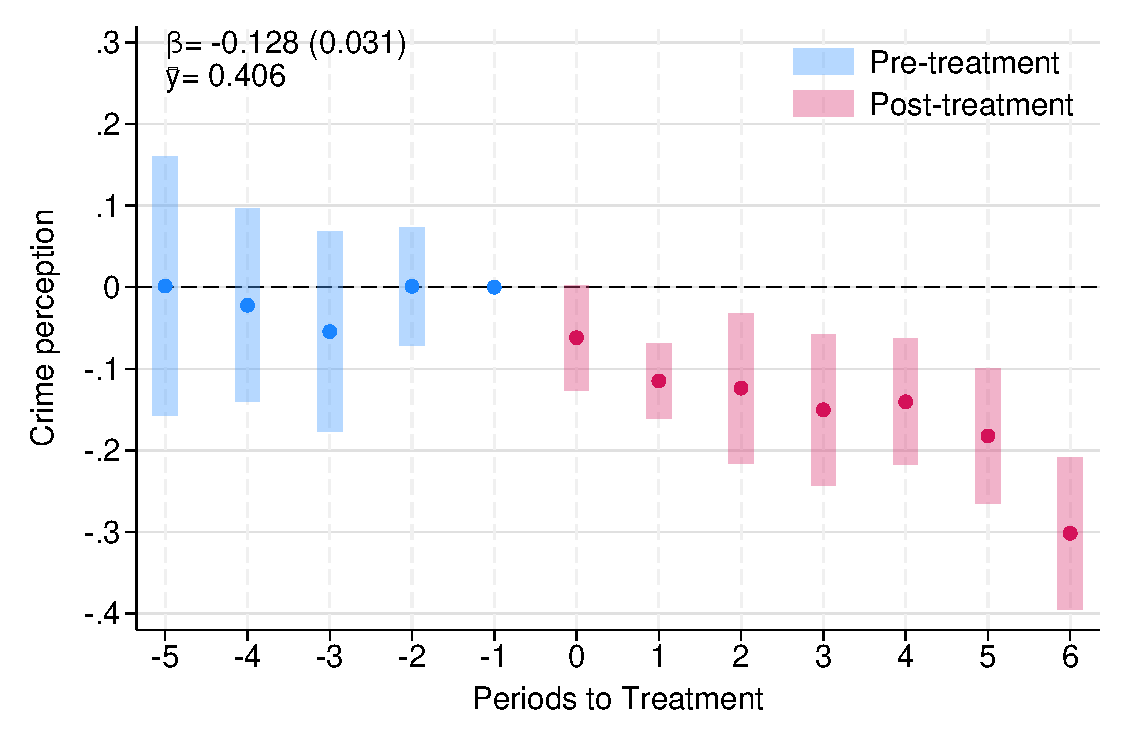
\includegraphics[width=\textwidth]{../manuscript/Graphs/results_perception_noEQ.pdf}
        \caption{Households reporting an increase in crime}
    \end{subfigure}%
    ~
    \begin{subfigure}{0.495\textwidth}
        \centering
        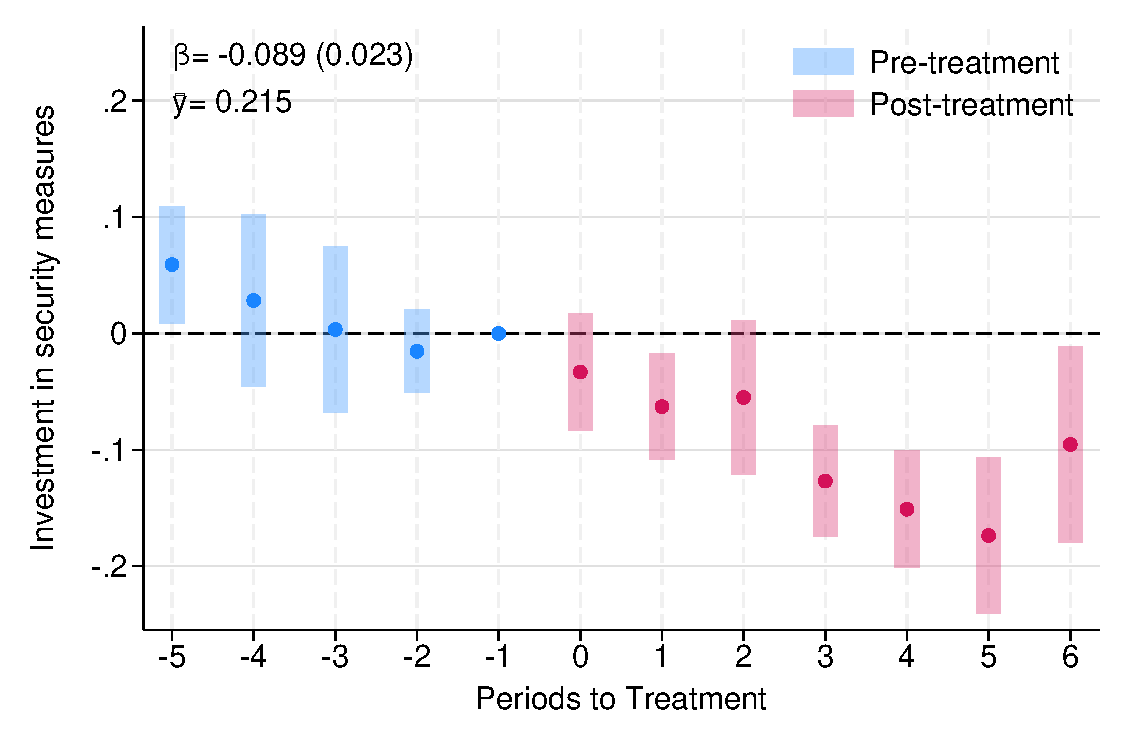
\includegraphics[width=\textwidth]{../manuscript/Graphs/results_hhprotectionmeasures_noEQ.pdf}
        \caption{Households adopting security measures}
    \end{subfigure}
    \\[12pt]
    \begin{minipage}{0.99\textwidth}
    \footnotesize
    Notes: This figure replicates the results of Figure \ref{fig:figure02} after excluding municipalities affected by the 2010 Maule earthquake, defined as those with a Modified Mercalli Intensity (MMI) score strictly greater than 7. The estimation is conducted using the procedure developed in \citet{Callaway} for difference-in-differences with staggered treatment adoption. The dots in the figure represent the estimated coefficients and the bars behind them 95\% confidence intervals. Standard errors are clustered at the municipality level using the wild bootstrapping procedure. The pooled effect and the mean outcome before the introduction of the treatment is also presented in each panel. Panel (a) reports the effect of \emph{Plan Cuadrante} on the probability of household victimization in the last 12 months using the ENUSC survey. Panel (b) reports the effect on the number of crimes reported to the police in the municipality per 100,000 inhabitants using administrative data. Panel (c) reports the effect on the probability of perceiving an increase in crime using the ENUSC survey. Panel (d) reports the effect on the probability of adopting security measures in the last twelve months using the ENUSC survey.
    \end{minipage}
\end{figure}
}


\begin{center}
{\renewcommand{\thefigure}{S1}
%--- Heterogeneity by exposure to the 2010 Maule earthquake (MMI > 7), all adopters
\begin{figure}[h!]
    \centering
    \caption{Effects of \emph{Plan Cuadrante} by Exposure to the 2010 Earthquake}
    \label{fig:heterogeneity_earthquake_mmi}
    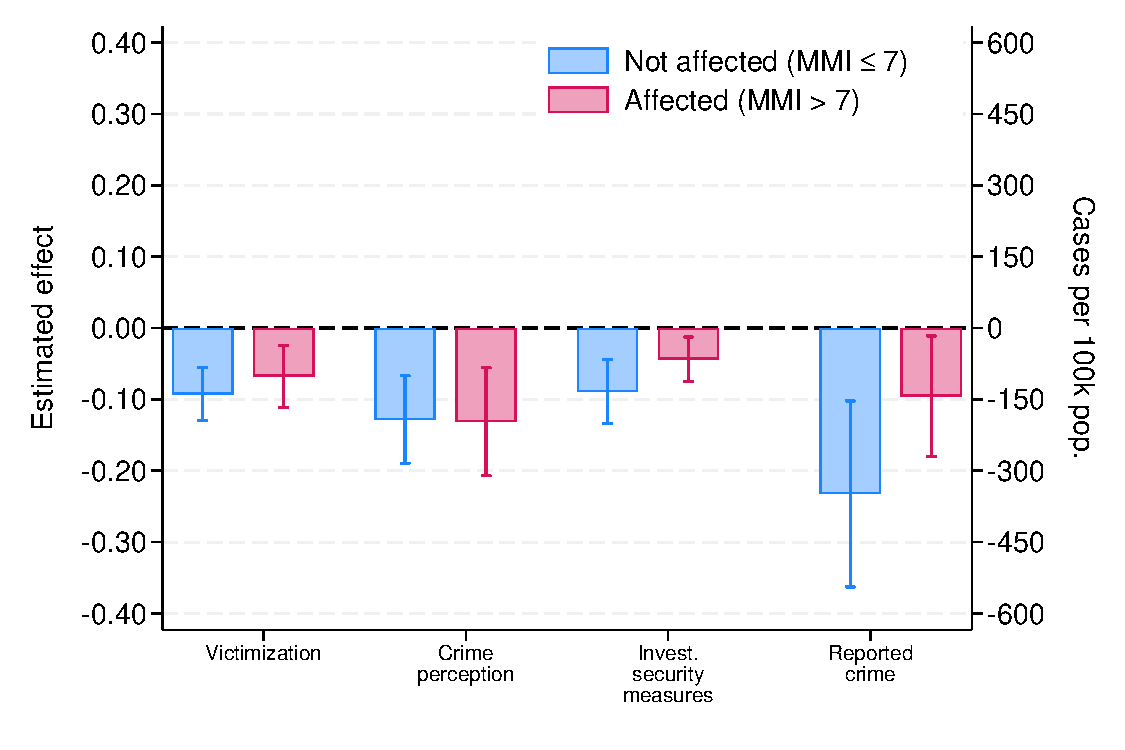
\includegraphics[width=0.8\textwidth]{../manuscript/Graphs/heterogeneity_earthquake_mmi.pdf}
    \\[10pt]
    \begin{minipage}{0.99\textwidth}
    \footnotesize
    Notes: This figure reports the heterogeneous effects of \emph{Plan Cuadrante} by exposure to the 2010 Maule earthquake, estimated separately for municipalities more exposed to the earthquake---defined as those with a Modified Mercalli Intensity (MMI) greater than 7, ``affected'' (red bars)---and municipalities with an MMI of 7 or lower (``not affected'', blue bars), using all adopters. For each exposure group, we estimate the pooled post-treatment effect of the program with the difference-in-differences estimator for staggered adoption of \citet{Callaway}, comparing municipalities of the same exposure level to each other so that the earthquake's direct effect on outcomes is differenced out within each group. Victimization is the probability of household victimization in the last 12 months; crime perception is the probability of perceiving an increase in crime; and investment in security measures is the probability of adopting security measures in the last twelve months---all from the ENUSC survey and read on the left axis. Reported crime is the number of crimes reported to the police per 100,000 inhabitants, from administrative data, and read on the right axis. Bars represent the average post-treatment effect and the whiskers the 95\% confidence intervals; standard errors are clustered at the municipality level using the wild bootstrapping procedure.
    \end{minipage}
\end{figure}
}
\end{center}


\clearpage